\section{The theorem prover E} \label{sec:c2s4}
\subsection{What is E}
\paragraph{}
E is a fully automatic theorem prover for \ac{fol} with equality implemented in ANSI-C that was released in 1998. Moreover, It is a saturation-based theorem prover. The Calculus implemented in E is variant of the superposition calculus proposed in \cite{BAGA94}.


\subsection{What can E do}
\paragraph{}
Since superposition calculus is a refutation one. So the current state of E, that it could prove the un-satisfiability of set of axioms with the negation of the conjecture(s) by finding the empty clause, or returning the saturated set if the empty clause was not found and no more new clauses can be inferenced/simplified. 


The returned saturated set is considered a model in the sense that it satisfies all the formulae in the give specification. However, an explicit model for the specification is not provided. Worth mentioning that it is not guaranteed in E to terminate/halt for \ac{epr} problems. This could be seen from the performance of E in \ac{epr} problems as it does not terminate in more than 50\% of them. 



\subsection{The Code flow of E}
\paragraph{}
This part is devoted from giving a brief on the main procedure in E. Figure \ref{fig:e_code_flow} is a simplified version of the code flow in E.

	\begin{figure}[H]
		\centering
		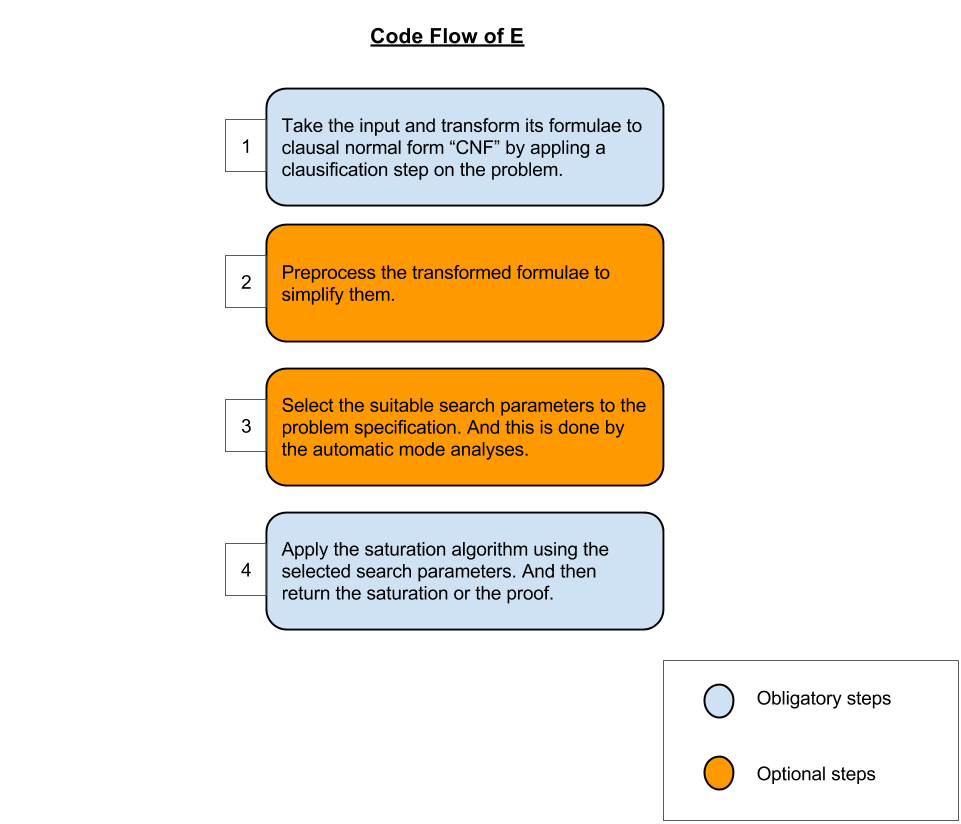
\includegraphics[scale=0.45]{pictures/e_code_flow.png}
		\caption{E Simplified code flow}\label{fig:e_code_flow}
	\end{figure}



\subsection{Latest results}
\paragraph{}
The latest results showed performance approaching 70\% over all the CNF and FOF problems of the TPTP problem set and this is according to \cite{E13}.